% AUTO-GENERATED by code/figlib.py helpers -- do not edit
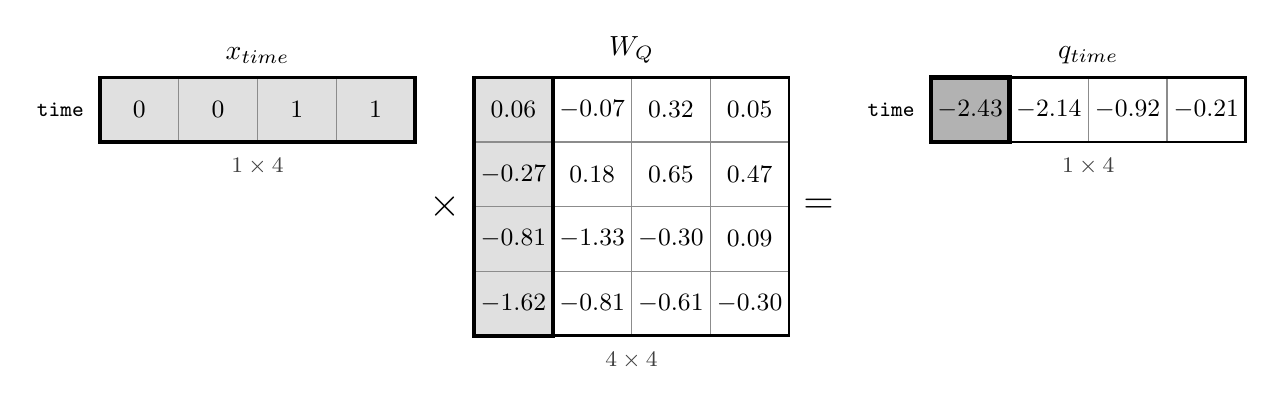
\begin{tikzpicture}
\draw[black!45, fill=black!12] (0.000,0.000) rectangle (1.000,-0.820);
\node[font=\small, text=black] at (0.500,-0.410) {$0$};
\draw[black!45, fill=black!12] (1.000,0.000) rectangle (2.000,-0.820);
\node[font=\small, text=black] at (1.500,-0.410) {$0$};
\draw[black!45, fill=black!12] (2.000,0.000) rectangle (3.000,-0.820);
\node[font=\small, text=black] at (2.500,-0.410) {$1$};
\draw[black!45, fill=black!12] (3.000,0.000) rectangle (4.000,-0.820);
\node[font=\small, text=black] at (3.500,-0.410) {$1$};
\draw[line width=1.4pt] (0.000,0.000) rectangle (4.000,-0.820);
\draw[line width=0.9pt] (0.000,0.000) rectangle (4.000,-0.820);
\node[anchor=east, font=\footnotesize\ttfamily] at (-0.080,-0.410) {time};
\node[anchor=south, font=\normalsize] at (2.000,0.050) {$\bm{x}_{\text{time}}$};
\node[anchor=north, font=\footnotesize, text=black!75] at (2.000,-0.900) {$1\times4$};
\draw[black!45, fill=black!12] (4.750,0.000) rectangle (5.750,-0.820);
\node[font=\small, text=black] at (5.250,-0.410) {$0.06$};
\draw[black!45, fill=white] (5.750,0.000) rectangle (6.750,-0.820);
\node[font=\small, text=black] at (6.250,-0.410) {$-0.07$};
\draw[black!45, fill=white] (6.750,0.000) rectangle (7.750,-0.820);
\node[font=\small, text=black] at (7.250,-0.410) {$0.32$};
\draw[black!45, fill=white] (7.750,0.000) rectangle (8.750,-0.820);
\node[font=\small, text=black] at (8.250,-0.410) {$0.05$};
\draw[black!45, fill=black!12] (4.750,-0.820) rectangle (5.750,-1.640);
\node[font=\small, text=black] at (5.250,-1.230) {$-0.27$};
\draw[black!45, fill=white] (5.750,-0.820) rectangle (6.750,-1.640);
\node[font=\small, text=black] at (6.250,-1.230) {$0.18$};
\draw[black!45, fill=white] (6.750,-0.820) rectangle (7.750,-1.640);
\node[font=\small, text=black] at (7.250,-1.230) {$0.65$};
\draw[black!45, fill=white] (7.750,-0.820) rectangle (8.750,-1.640);
\node[font=\small, text=black] at (8.250,-1.230) {$0.47$};
\draw[black!45, fill=black!12] (4.750,-1.640) rectangle (5.750,-2.460);
\node[font=\small, text=black] at (5.250,-2.050) {$-0.81$};
\draw[black!45, fill=white] (5.750,-1.640) rectangle (6.750,-2.460);
\node[font=\small, text=black] at (6.250,-2.050) {$-1.33$};
\draw[black!45, fill=white] (6.750,-1.640) rectangle (7.750,-2.460);
\node[font=\small, text=black] at (7.250,-2.050) {$-0.30$};
\draw[black!45, fill=white] (7.750,-1.640) rectangle (8.750,-2.460);
\node[font=\small, text=black] at (8.250,-2.050) {$0.09$};
\draw[black!45, fill=black!12] (4.750,-2.460) rectangle (5.750,-3.280);
\node[font=\small, text=black] at (5.250,-2.870) {$-1.62$};
\draw[black!45, fill=white] (5.750,-2.460) rectangle (6.750,-3.280);
\node[font=\small, text=black] at (6.250,-2.870) {$-0.81$};
\draw[black!45, fill=white] (6.750,-2.460) rectangle (7.750,-3.280);
\node[font=\small, text=black] at (7.250,-2.870) {$-0.61$};
\draw[black!45, fill=white] (7.750,-2.460) rectangle (8.750,-3.280);
\node[font=\small, text=black] at (8.250,-2.870) {$-0.30$};
\draw[line width=1.4pt] (4.750,0.000) rectangle (5.750,-3.280);
\draw[line width=0.9pt] (4.750,0.000) rectangle (8.750,-3.280);
\node[anchor=south, font=\normalsize] at (6.750,0.050) {$W_Q$};
\node[anchor=north, font=\footnotesize, text=black!75] at (6.750,-3.360) {$4\times4$};
\draw[black!45, fill=black!30] (10.550,0.000) rectangle (11.550,-0.820);
\node[font=\small, text=black] at (11.050,-0.410) {$-2.43$};
\draw[black!45, fill=white] (11.550,0.000) rectangle (12.550,-0.820);
\node[font=\small, text=black] at (12.050,-0.410) {$-2.14$};
\draw[black!45, fill=white] (12.550,0.000) rectangle (13.550,-0.820);
\node[font=\small, text=black] at (13.050,-0.410) {$-0.92$};
\draw[black!45, fill=white] (13.550,0.000) rectangle (14.550,-0.820);
\node[font=\small, text=black] at (14.050,-0.410) {$-0.21$};
\draw[line width=1.6pt] (10.550,0.000) rectangle (11.550,-0.820);
\draw[line width=0.9pt] (10.550,0.000) rectangle (14.550,-0.820);
\node[anchor=east, font=\footnotesize\ttfamily] at (10.470,-0.410) {time};
\node[anchor=south, font=\normalsize] at (12.550,0.050) {$\bm{q}_{\text{time}}$};
\node[anchor=north, font=\footnotesize, text=black!75] at (12.550,-0.900) {$1\times4$};
\node[font=\Large] at (4.375,-1.640) {$\times$};
\node[font=\Large] at (9.125,-1.640) {$=$};
\end{tikzpicture}
